%!TEX root = ../thesis.tex
%\begin{savequote}[75mm]
%Nulla facilisi. In vel sem. Morbi id urna in diam dignissim feugiat. Proin molestie tortor eu velit. Aliquam erat volutpat. Nullam ultrices, diam tempus vulputate egestas, eros pede varius leo.
%\qauthor{Quoteauthor Lastname}
%\end{savequote}

%\chapter{\textsc{The internship project}}
\chapter{The internship project}

%\newthought{There's something to be said} for having a good opening line. Morbi commodo, ipsum sed pharetra gravida, orci  $x = 1/\alpha$ magna rhoncus neque, id pulvinar odio lorem non turpis \cite{Eigen1971, Knuth1968}. Nullam sit amet enim. Suspendisse id velit vitae ligula volutpat condimentum. Aliquam erat volutpat. Sed quis velit. Nulla facilisi. Nulla libero. Vivamus pharetra posuere sapien. Nam consectetuer. Sed aliquam, nunc eget euismod ullamcorper, lectus nunc ullamcorper orci, fermentum bibendum enim nibh eget ipsum. Donec porttitor ligula eu dolor. Maecenas vitae nulla consequat libero cursus venenatis. Nam magna enim, accumsan eu, blandit sed, blandit a, eros.
%$$\zeta = \frac{1039}{\pi}$$

% For an example of a full page figure, see Fig.~\ref{fig:myFullPageFigure}.

This chapter contains the results of the discussions and planification that have been made prior to the beginning of the internship.
These contents are described in more detail in the Piano di Lavoro, a document that contains an estimation of resources for each task that composes the project.

At the beginning of May I have met the tutor in order to understand what the company wants and make a first time planification.

In here is also described how a resolution for the problem was first thought.

\section{The company's needs}

	As said earlier Athonet is a growing company.
	At the time of writing it has nearly 40 employees and it is expected to hire new people for open positions.
	Athonet uses multiple software tools for keeping track of projects, sharing information internally and with the clients, visualizing product roadmaps, etc.
	The most important tools they are currently relying on are:
	\begin{itemize}
		\item Redmine as an Issue Tracking System
		\item SharePoint as a collaborative platform
		\item Planner for visualizing project roadmaps
		\item GitLab as a repository
	\end{itemize}
	Not all of these have been created with the idea of being used together.
	There are plugins that connect them, but these don't allow much customization and since are made from multiple developers, not always are compatible when a new software release is issued.
	There is a need then to provide employees with a suite of stable tools that are easily interconnected and with a vast and well done documentation.
	Also, these tools must be easy to maintain and update, since they don't have to become obsolete and outdated.
	Nobody likes legacy systems.
	
	%todo dilbert legacy system comic strip
	
	Internal changes may not be directly visible to the clients, but the effect of having a much organized company, where there is always track of the work done and in progress ensures that when there is a request from the client it does not go unseen or unanswered.	
	Forcing employees to use a software instead of another one though is not easy without creating chaos.
	This is why a good and easy to consult documentation is the key on helping employees transition.

\section{Requirements and objectives}

	When discussing with the tutor he as explained me the problem step by step and we have set some requirements in order to give them importance and priority.
	The final objective was to create a suitable environment that would work and be ready to transfer it into production and explain the users how to use it.	

	Requirements can be divided in three categories based on their importance:
	\begin{itemize}
		\item Mandatory (Obbligatorio in italian): that have to be implemented, represent the core of the project
		\item Desirable (Desiderabile in italian): not mandatory for the final objective but add greater value
		\item Optional (Facoltativo in italian): add value to the project but not as much as the previous ones, carried out only if there is time left for them
	\end{itemize}

	Each requirement has a unique ID that is composed by the first letter of their importance (from the italian word to resemble the Piano di Lavoro) and a number.

	\hl{Here a list of the requirements, as presented in the work plan document:}

	%todo aggiungere tabella con i requisiti

\section{Approaching the problem}

	How I thought I could approach the problem.
	Write that I have thought of use chases and associate them to the requirement?

\section{Time division and planning}

	To formalize the time division of the project I have used a Gantt diagram and a table contains a realistic approximation of the hours spent per task.
	The internship was planned for ten weeks, which is a little more than two months, and the project has been spread such that I could have time to understand the tools and use them so that I could get acquainted.
	This time period also includes the phases for getting feedback from users, fine tune the configuration, explain the tools to various members of the company and, in case of incidents, slack time.
	\begin{figure}[H]
		\centering
		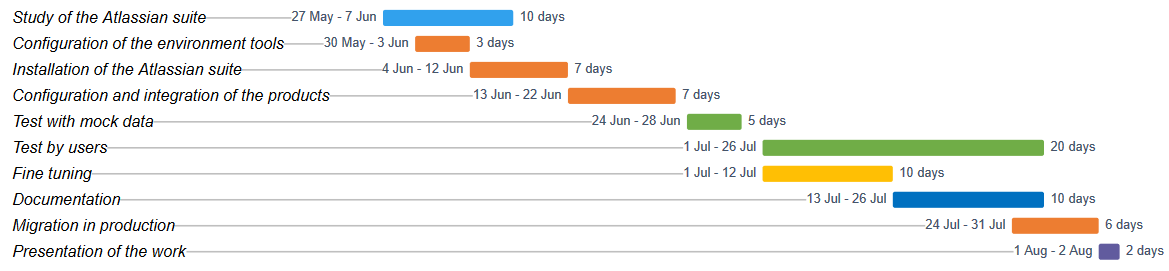
\includegraphics[width=1.1\textwidth]{resources/work_plan_gantt}\\
		\caption{Gantt diagram contained in the ``\textit{Piano di Lavoro}'' document}
	\end{figure}
	I started to create a temporal sequence only after I well understood the requirements and got an idea about how Atlassian's software works.
	To create a good plan I have started from understanding what was the final objective and asking myself the question of how can I achieve it.
	
	% todo spiegare diagramma di gantt?
	
	I have coarse grained planned four main time periods:
	\begin{itemize}
		\item Learning
		\item Implementing
		\item Testing
		\item Feedback
	\end{itemize}
	
	Each of these contain smaller tasks that involve studying the tools, installing them and configuring them.
	As discussed with the tutor, meetings had to be considered so that I could explain the progress to him and to other company figures that would eventually use the software.
	
	As milestones / baselines I considered having a deliverable that could be easily transitioned from the development to the production environment, such as a script that installs and configures the software or a container.
	By definition this must be versionable and with a well written changelog.
	
	